\section{SmolLM3 Diagnostics and Capability Evaluation}
\label{app:smollm_diagnostics}

\subsection{Checkpoints, responses, and weighting}

We use the SmolLM3-3B MixSFT student, three domain-specific RL teachers, and exported 500-update students for I64-DR/DT/GT and PG-DR/SGD. The model and data revisions, export hashes, and diagnostic source snapshots are recorded with the measurements. The reported I64 training configurations use Adam with learning rate $2.5\times10^{-7}$; PG uses SGD with learning rate $0.0025$. The capability comparison uses a new shared evaluation protocol.

Diagnostic prompts come from the frozen Open-MOPD data revision \texttt{9e897efe}, with unique raw messages shuffled within mathematics, code, and instruction following. Coverage, normalization, and probe prompt splits are disjoint within this diagnostic sample. We preserve dataset messages and disable thinking in the chat template. Generation uses temperature 1, top-$p=1$, a 2,048-token prompt cap, and a 4,096-token response cap. Each natural coverage bank contains 384 responses, 128 per domain, with up to eight uniformly spaced positions per response: 3,053 prefixes for MixSFT and 3,058 for DR500. Additional students score the same 3,058 DR500 prefixes without regenerating responses.

Coverage statistics assign equal weight to domains, responses within domains, and audited positions within a response. Mean-mass intervals resample responses independently within each domain 2,000 times using seed 1042/1043/1044. MixSFT and DR500 use their own natural banks; the remaining students use the DR500 bank. The minimum I64 mass on DR500's natural bank is $1.7\times10^{-8}$; DT500 and GT500 each have one empty intersection in the common-bank audit.

\subsection{Frozen subsets and gradient comparisons}

Within each domain we select representative prefixes, prefixes above its 75th entropy percentile, and prefixes with I64 mass below 0.99. Selection allows overlap between strata and uses up to 32 distinct prompts per domain. The low-coverage code stratum has 21 eligible prompts, yielding 85 distinct prefixes overall. Each stratum is divided into three batches. Small candidate budgets $k=4,8$ are selected by a coverage-only rule.

The BF16 coverage audit sorts a top-128 list and takes its first $k$ entries, whereas gradient diagnostics recompute top-$k$ directly in FP32 at the exported BF16 parameter values. Student forward/backward passes use FP32; cached teacher targets use BF16 forward passes followed by FP32 log-softmax. One of the 85 frozen low-coverage prefixes crosses 0.99 during the FP32 diagnostic and remains in its original stratum. The FP32 diagnostic mean I64 masses are 99.05\%, 95.68\%, and 93.12\% for the representative, high-entropy, and low-coverage groups.

Full KL, PG, and intersection objectives use the definitions in Appendix~\ref{app:losses}. Empty intersections produce zero loss. We retain zero- and small-norm cases and report vector differences in addition to cosine. The plotted relative error is $\|g_{I_k}-g_{\mathrm{full}}\|/\|g_{\mathrm{full}}\|$, which measures the vector difference relative to the full-vocabulary gradient norm.


\subsection{Cumulative BF16 changes by parameter group}

The exported MixSFT-to-DR500 comparison contains 3,075,098,624 unique parameter coordinates after accounting for tied embeddings. The 36 transformer blocks each contain 78,123,008 coordinates, the token embedding 262,668,288, and the final normalization 2,048. We compare the two BF16 exports directly. Overall, 10.47\% of coordinates change; the largest 1\% carry 36.85\% of squared displacement, and 5.85\% of coordinates carry 90\%. Figure~\ref{fig:smollm_cumulative} retains all parameter groups. Per-group changed fractions use each group's own coordinate count; displacement shares use total model squared displacement.

\begin{figure}[p]
\centering
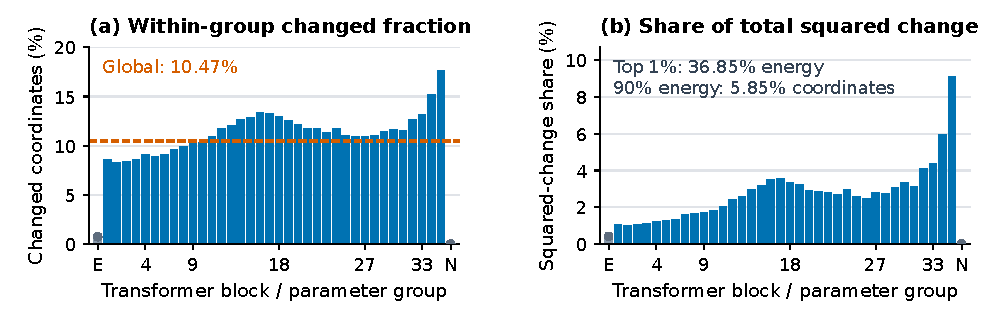
\includegraphics[width=\linewidth]{figures/visual_mvp_20260918/smollm_cumulative.pdf}
\caption{\textbf{Cumulative BF16 changes differ across all 38 SmolLM3 parameter groups.}
MixSFT to DR500: blocks 0--35, embedding (E), final norm (N). (a) Within-group changed fraction; dashed: global parameter-weighted fraction. (b) Share of total squared displacement. Tied weights count once.}
\label{fig:smollm_cumulative}
\end{figure}
